\chapter{Discussion}
\label{chap:discussion}

\section{Combining the Six Agents with a Single Regression Model}
In the clustering player approach, in order to have a fair comparison with the baseline that uses only a single predictor, we decided to use six linear models and combine their predictions afterwards. However, we experimented also to use a single linear model that takes as input all the six agents' \acs{sr}. We found that this model has a very similar MAE and MSE of our approach. However, looking at the p-value of each predictor we found that agent 2 has a p-value of 0.61, meaning that its predictions are not improving the model and they might be highly correlated to other agents' predictions. By removing this agent from our approach, we found that all the remaining predictors have a p-value that is lower than 5\% while the performance of the approach remained unchanged. A similar result is obtained in the clustering simulated strategies approach. The lowest p-value between the six predictors was 0.08 and removing the corresponding agent did not alter the results. This is beneficial not only for simplicity, but also for sustainability, since each time a new game content needs to be tested we have to simulate gameplay with all the developed agents. By reducing the number of simulations we will reduce the computational resources utilized. Furthermore, by providing more accurate predictions, our approaches can reduce the number of iterations required by game designers to adjust a level. However, we need to consider that the computational requirements of our approach grow linearly with the number of simulated groups of players. From the sustainability point of view, a deeper analysis of the trade-off between number of iterations and number of simulations per iteration is necessary to answer if the proposed approach is more or less sustainable than the baseline approach. Finally, since the various simulations can be executed in parallel the time required to test a game content is the same as the baseline approach.


\section{Comparison of the Two Approaches}

Even if it is not the purpose of this thesis a comparison between the two approaches may be of interest. Nevertheless, we need to remind that the agents in the two approaches are trained on different data sets and predict on different test levels.
By looking at the comparison of the two approaches with the baseline, we observe that they produce very similar improvements in the linear part. On the contrary, if we consider both the linear predictions and the mean predictions the clustering players approach only slightly improve the baseline yet being better in absolute numbers than the clustering simulated strategies approach. However, the diversity may be due to the different test levels considered in the two approaches. Note that in the clustering players approach we had to remove levels that drastically changed during time. Indeed, comparing the two approaches with the same test levels we obtained similar results.
The clustering players approach favors description and interpretation, meaning that the various agents directly simulate a specific group of players. This means that if a particular behaviour is discovered by the simulation of an agent, it is possible to go back to the players that showed this behaviour. However, it requires that meaningful player clusters are created and more importantly, that players in different clusters use, on average, different strategies. On the contrary, the clustering simulated strategy approach works better when the relationship between player features and strategies is unknown. By looking at the player features of the selected agents, it is possible to qualitatively determine which player each generated agent represents. Furthermore, during training, this approach uses all the available data and should be preferred when gameplay data are limited. However, one of the major drawback of this approach is that the feature combinations tested to select the agents grow exponentially with the number of player features. A possible solution could be to randomly select few of them or use evolutionary algorithm to explore the feature space and select the agents. In this research we aimed to model different type of players and as a consequence we selected the agents that led to more diverse strategies, however, it may be of interest to select agents based on their performance in the game or other metrics.


\section{Practical Implications}

Accurately determining the difficulty of a level is crucial for game companies since the difficulty has an impact on the revenues, both directly, in terms of boosters bought by the players and indirectly, in terms of player satisfaction and entertainment. For example, if a too difficult level is included in the game, there is a risk that frustrated players may stop playing the game. Furthermore, being able to estimate the perceived difficulty of a specific group of players, can provide an indication of how many players could be affected by a too difficult level. Additionally, it allows game designer to create levels with a desired difficulty for specific players. As an example, a game designer may want to create a level that is easy for everyone while another game designer may want to develop a level that is easier for regular players than for occasional players. 
Furthermore, it is possible to allow the \acs{CNN}-based agents to play extra moves after the maximum number of available moves is reached. Since the maximum number of moves is a parameter that game designers need to decide when creating a level, simulating longer gameplay allows to compute an estimate of how many moves to add if a level is considered too difficult for a specific type of players or globally too difficult. Furthermore, since players have the possibility to buy boosters that give them extra moves at the end of an attempt, we can estimate the potential impact of this type of boosters on different players. 

The experiments in this thesis were performed using a cloud service provider. Thanks to the fact that the training of the agents and the simulation of the gameplay can be executed in parallel, the proposed approaches scale very well with an increase of computational power. Furthermore, not only the simulation of different agents were executed in parallel, but for each agent, several copies were executed, each one simulating several attempts of the same level. As a consequence, we experimented using 1,000 attempts per level and preliminary results showed a little improvement of the players' \acs{sr} prediction.
Finally, a deeper analysis on the agents' performance discovered that for levels that contain a special item called "Sugar Key", the agents' \acs{sr} is constantly lower than the players \acs{sr}. The "Sugar Key" are key-shaped candies, which can be matched like regular candies, however they cannot be matched with any special candy. The "Sugar Key" is always present with one or more "Sugar Chest". Every time a key is destroyed, a layer of lock on the chests is removed. Removing all the chests is usually a necessary condition to complete the level. As a consequence, the lower agents' performance can be explained by the fact that a different or deeper \textit{strategic thinking} is required when this element is present on the game board, or it might be a lack of training data with these special items since they appear only on 8\% of the levels. Also the "Sugar Key" can appear in six different colors and for each color it is considered as a different input feature for the \acs{CNN}. A deeper analysis is necessary to better understand this issue.

\section{Generalization of the Results}
Despite the fact that we tested our approaches using the \textit{Candy Crush Saga} game, we believe that the same approaches, with few variations, can be applied to other games as well. Using player features to differentiate gameplay simulations and better predict players' behaviour is a general concept that can apply to many games. Furthermore, the proposed approaches could have an even bigger impact on those games where the features of the players have a stronger relationship with the player strategies \cite{holmgard_evolving_2014}. 
% For example, in a shooting game, a player that uses an handgun (player features), probably runs and shots more frequently compared to a player that uses a sniper rifle. In this case, since the relationship between player feature and actions is stronger may be captured better by the prediction model.

\textcite{drachen_guns_2012} in their research, showed how the selection of the clustering algorithm can lead to different insights of the players population. In the clustering players approach, we used k-means to extract the general distribution of players' behaviour. By using others clustering algorithms, like Simplex Volume Maximization, we could identify and model players with extremes behaviours and use them to obtain different insights about the game. Furthermore, as illustrated by \textcite{holmgard_evolving_2016}, the developed agents could be useful to characterize and classify new players by looking at which agent better represents the player decision making style.
In this thesis we focused on the players' \acs{sr} as a metric to evaluate new game content. However, the proposed approaches can be used to estimate other metrics. As an example, in \textit{Candy Crush Saga}, we can use the developed agents to estimate the score distribution and automatically set the thresholds for reaching one, two or three stars on each level. These parameters are usually set and fine-tuned by game designers.
Moreover, especially in other games, the proposed approaches could also work with completely different metrics.

Finally, the developed agents can be used for several purposes. Similarly to what \textcite{holmgard_evolving_2014} did in their research we can visualize the gameplay simulation to observe how different players interact with the game or we can use the agents to perform game balancing \cite{hunicke_case_2005}, providing each player with a slightly different level that matches their performances, skills and expectations.

\section{Limitations}
In this thesis, due to the properties of the experimented game, we used player features that are indirectly related to the player strategies. Defining, tracking and computing player features that directly relate to the performed moves, e.g. number of special candies created, could be useful to improve the developed player models. Moreover, in this work we did not consider the direction of the performed moves. Adding the possibility for the agents to chose between left-right or right-left moves and top-down or bottom-up moves can potentially increase the performances of the developed agents. Furthermore, we could also add the possibility for the agents to use in-level boosters by increasing their action space.
Another possible limitation is that the presented approaches can only be used in games where the content evolves during time since they use data from existing game content to predict on future ones. Nevertheless, in most of the \acs{F2P} games the game content is continuously added in order to engage and retain players. In addition, since we simulate gameplay using \acs{CNN}-based agents, the experimented approaches work better with games that have states that can be represented with images or encoded in a grid-shape topology, games that have a discretizable action space and games that have the Markov property. Finally, a last limitation regards the models used to predict the players' \acs{sr}. In this thesis, we used linear regression models. However, using more complex models could improve the prediction performances and a possible approach is discussed in the next section.  

\section{Future Work}

\subsection{Players' SR Prediction with Generalized Linear Models}
To overcome the limitations of the linear regression models in the players' \acs{sr} prediction stage we could try to use \acfp{GLM}. \acsp{GLM} are helpful, especially when the range of the dependent variable $y$ is restricted and the variance is not the same along the predicted values but depends on the mean of $y$. A generalized linear model is built with a linear predictor and two functions: a link function describing how the mean of $y$ depends on the predictor and a variance function describing how the variance depends on the mean. The general linear regression applied in this research is a particular case of \acs{GLM} with identity link function and unit variance. In our case, since the predicted \acs{sr} is a ratio and assumes values between 0 and 1, it could be better modeled by a binomial distribution. As a consequence a possible approach could be to use a \acs{GLM} with \textit{logit} as link function and variance function $V(\mu_i)$ defined as:
\begin{equation}
    V(\mu_i) = \mu_i(1 - \mu_i) \text{,}
\end{equation}
where $\mu_i$ is the expected value of $y$.
A preliminary experiment showed that a \acs{GLM} with binomial distribution improves the \acs{MAE} of both the proposed approaches.
Furthermore, it could be worth to model the extra uncertainty that derives from the fact that the agents play deterministically and as a consequence the agent's \acs{sr} is self-correlated. Meaning that there are some levels where the agent is always good or always bad while when we aggregate the players we average between different \acs{sr}. More work in this direction could be done to improve the performances of the proposed approaches.


\subsection{Further Applications}
The benefits of having multiple agents simulating different strategies are not limited to better estimate the players' \acs{sr} on new levels. A first extension is to compute different metrics while other applications are reported in this section and future work should deepen these aspects.

\subsubsection*{Clean the data}
 
While tracking gameplay data from players we are aware that also "noise" in the data is tracked as well. As an example, sometimes players might select moves randomly, without focusing on the game and this data are tracked as well. Having multiple agents simulating different strategies could be beneficial to reduce this noise. Our approaches help to directly model the diversity in the player strategies. However, while modeling player strategies we inevitably include the tracked "noise" in the simulated behaviour. This is especially true for casual games that can be played without too much concentration. A possible approach to discover moves that are selected randomly, is to look at the time spent by the players to select each move and compare it with the average time spent. If a move is selected very fast, this could indicate that it is just picked randomly.
Furthermore, some gameplay data are more useful to learn different player strategies than others.
If all the agents predict the same move, this means that independently from which strategy they simulate the players more likely select that specific move. Results showed that 23\% of the time all the developed agents predict the same move. It could indicate that these are states where a specific move is clearly preferred by the players. Maybe because there is only one legal move available or maybe because the predicted move leads to win the game. Since no difference is learnt from the \acsp{CNN} in these states, removing them and re-training the networks could potentially increase the differences in the simulated strategies.
Finally, we need to consider that we are simulating the strategies of groups of players and not individual ones. As a consequence it is possible that two different players, even if they belong to the same cluster, select two different moves in a given state. It is also possible that a player selects different moves even in the exact same state in two different moments. Note that in the experimented game it is hard to decide which move leads to the best outcome. By looking at the predicted probability of the \acs{CNN} we can detect the gameplay data where the network is not sure on which move is the best one. As an example we can set a threshold and if the network predicts two or more moves with probabilities that differ less than the threshold we can assume that the network is not able to decide which one is preferred and a different strategy to select the move might be appropriate in this case. In order to simulate different strategies of the same group of players we can select from the distribution of the predicted moves using different policies instead of the greedy one. This means that for example, if a move is scored $0.2$ by the \acs{CNN}, it will be selected with probability of 20\%. The \textit{softmax} function applied by the output layer guarantees that the predicted scores can be interpreted as probabilities and sum up to one. However, previous experiments showed that selecting moves in a non-greedy manner, only lead to worse performances. Future work in these directions is needed to validate or reject our hypothesis and deeper understand both the players and the game.


\subsubsection*{Categorize levels}
A possible application is to categorize levels based on the strategy required to solve them, similarly to what \textcite{isaksen_simulating_2017} have done with \textit{Tetris} and \textit{Puzzle Bubble}. The idea is to create a population of different agents each one with a different strategy level. Furthermore, the generated population can be extended by adding "strategy errors". Instead of selecting the moves with a greedy strategy, is possible to use an $\epsilon$-greedy strategy where the $\epsilon$ parameter defines how frequently each agent makes an error. The error is performed by selecting a random move instead of the one predicted by the model. Then, by comparing the performances of the agents, is possible to estimate the strategy required by each level. This approach is built on the assumption that the strategy learnt from player data is enough to solve the level. Nevertheless, we observed that on average, 82\% of the tested levels are successfully completed by the agents. 
We performed a preliminary analysis to categorize levels based on the strategy required to solve them. To obtain a meaningful analysis we restricted our focus to those levels that are successfully solved by the agent when playing with no strategy errors, using the greedy policy. We created a population of 16 different agents, each one simulating a different amount of strategy error. We randomly selected 20 levels to test this approach and we ordered the agents from the one that plays completely random (\textit{$\epsilon$ = 1}) to the one that plays greedily (\textit{$\epsilon$ = 0}). By plotting the agent's \acs{sr} against the amount of strategy used, represented by \textit{$1 - \epsilon$}, we observed how the \acs{sr} improves as we reduce the number of random moves performed. Figure \ref{fig:two_levels_strategy} shows for two levels the amount of strategy used by the agent plotted against the agents' \acs{sr}. A strategy level of zero means that the agent uses a random policy while a strategy level of one means that the agent follows a greedy policy. Note that the agents' \acs{sr} are normalized dividing them by the maximum value. This because in order to compare levels, we assume that when the agents play with full strategy they reach the optimal performances ($SR = 1$).
\begin{figure}[h]
  \centering
  \subfloat[]{%Level 154
    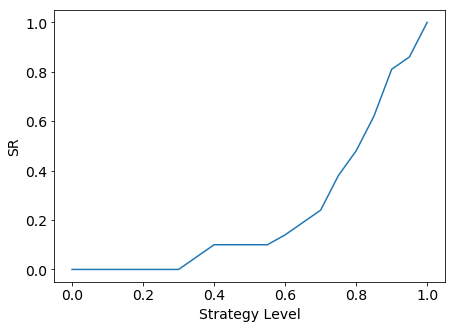
\includegraphics[width=0.45\textwidth]{masters-thesis-master/masters-thesis/contents/05_discussion/strategy_req/154.png}
    \label{fig:154}
    }
    \subfloat[]{%Level 155
    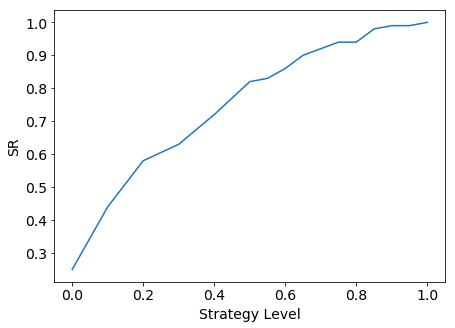
\includegraphics[width=0.45\textwidth]{masters-thesis-master/masters-thesis/contents/05_discussion/strategy_req/155.png}
    \label{fig:155}
    }
    
    \caption{Two examples of strategy requirement plots for two random levels. Figure (a) shows a level (number 154) that has a high strategy requirement while (b) shows a level (number 155) that requires less strategy to be solved. The \acs{sr} on the y-axis is normalized dividing it by the maximum value.}
    \label{fig:two_levels_strategy}
\end{figure}
To estimate the strategy required by a level we propose to use the area above the line. This metric indicates how much strategy is required to complete the levels. In the two extreme cases, the area above the line is zero when no strategy is required and the \acs{sr} is constantly equal to one independently of the amount of random moves. On the contrary, the strategy required is one when the optimal strategy is needed to solve the level and the \acs{sr} is constantly zero except for the agent that plays greedily. Having different metrics to evaluate a level can be useful for game designers to test the levels and to improve the quality of the game. Finally, we can hypothesize that levels that can be successfully solved also with random moves might be perceived less challenging by some players or that levels that require too much strategy might be an obstacle to some other players. A deeper analysis is needed to verify these hypothesis. 

In their research, \textcite{isaksen_simulating_2017} also estimated the dexterity required by each level. However the motor-skill required to correctly perform a move in \textit{Candy Crush Saga} are very low and levels that require a lot of dexterity do not exist. Nevertheless, if the proposed approaches are applied to other games it may be valuable to estimate the dexterity requirement too. Regarding \textit{Candy Crush Saga} a slightly different ability, called observability, can be modeled and estimated on each level. The idea is that players, differently from the developed agents, do not always detect all the available moves on the game board. We can add this type of error to the agents in different quantities and then estimate the observability required by each level. The error can be modeled by randomly reducing the number of available moves that the agent can select. The moves will not be selected randomly as it is for the strategy error, instead they will be selected greedily but within a subset of all the available moves. As an example, an observability of 50\% means that the agent only detects half of the available moves on each game board. As a consequence if the agent predicts a move that is not between the ones that are detected, the move is discarded and the subsequent predicted move is selected. This process is repeated until the predicted move is in the subset of the detected moves. Moreover, instead of randomly detecting the moves, different heuristics can be used to decide which moves are detected and which ones are not. As an example, we can create an agent that more often detect matches of red candies than blue candies or an agent that more often detect matches with T-shape rather than L-shape. Ideally, we could learn also these peculiarities from data.

Another application might be to classify each level based on the agreement between the agents in selecting the moves on game boards obtained from that level.
Computing the agents' agreement on several game states obtained from a specific level allows us to categorize levels based on how often different agents agree. The idea is that levels where all the agents select the same moves are less fun to play since the player strategy has a minor impact on the gameplay.
Finally, we can also categorize levels based on the predicted probabilities of the network \cite{costa_probabilistic_1996}. For example, if the network on a specific level consistently predicts a move with high probability it might indicate that the possible choices for the player are limited and as a consequence the level is less entertaining, while on the contrary if the network predicts many moves with similar probabilities it might indicate a more fun and challenging level.


% \subsection{Three Sources of Noise}
% The proposed approaches allow us to deeper understand what we call "the three source of noise" in the gameplay data. 

% First, players uses different strategies, second,  Third, even if a player is focused on selecting the best move,  Since these are properties of the players, gameplay simulation with player modeling mimics these behaviour as well. Being able to model and separate these three components might be useful to obtain better analysis. 

 
% Regarding the difficulty of evaluating the moves, we can look at the prediction accuracy of the networks. Despite the fact that we select the move with the highest accuracy, if a move is predicted with high accuracy we can say that this move is clearly perceived better than the others moves, at least from the player perspective. On the contrary, if two moves are predicted with equal probability, these could indicate that also for players is hard to evaluate which one is better.









